\documentclass[12pt]{article}
%\pagestyle{empty}
% NMD additions 
%\usepackage{graphicx, overpic}
\usepackage[colorlinks=true, linkcolor=blue, citecolor=blue]{hyperref}

% end NMD additions 
\usepackage[T1]{fontenc}

 \setlength{\tabcolsep}{20pt}
\setlength{\topmargin}{0.5cm}
\setlength{\oddsidemargin}{-0.2cm}
\setlength{\evensidemargin}{-0.2cm}
\textheight = 22cm  
\textwidth = 16.2cm


\usepackage{enumerate, amsfonts, latexsym, color, url}
\usepackage[pdftex]{graphicx}
%\usepackage{epstopdf}

%\usepackage{pinlabel}


\begin{document}


\title{{\tt wireframe}; a simple program for drawing surfaces}

\author{Danny Calegari}
%\address{University of Chicago \\ Chicago, Ill 60637 USA}
%\email{dannyc@math.uchicago.edu}
\date{\today}


%\begin{abstract}
%\end{abstract}

\maketitle
\setcounter{tocdepth}{1}
\tableofcontents

\section{Summary}
This manual describes the X-windows program {\tt wireframe} and the format of the data files it takes.
This program can be used to easily create .eps figures of rendered three-dimensional surfaces
for inclusion in scientific articles.

\begin{figure}[ht]
  \caption{A once-punctured torus in {\tt shaded} mode}\label{punct}
  \centering
    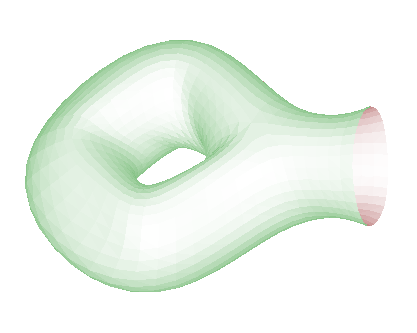
\includegraphics[width=0.5\textwidth]{punct}
\end{figure}

Figure~\ref{punct}
gives an example of a once-punctured torus in {\tt shaded} mode.
Figure~\ref{braid_iso} gives an example of a closed braided surface in {\tt isobar} mode. 

\begin{figure}[ht]
  \caption{A braided surface in {\tt isobar} mode}\label{braid_iso}
  \centering
    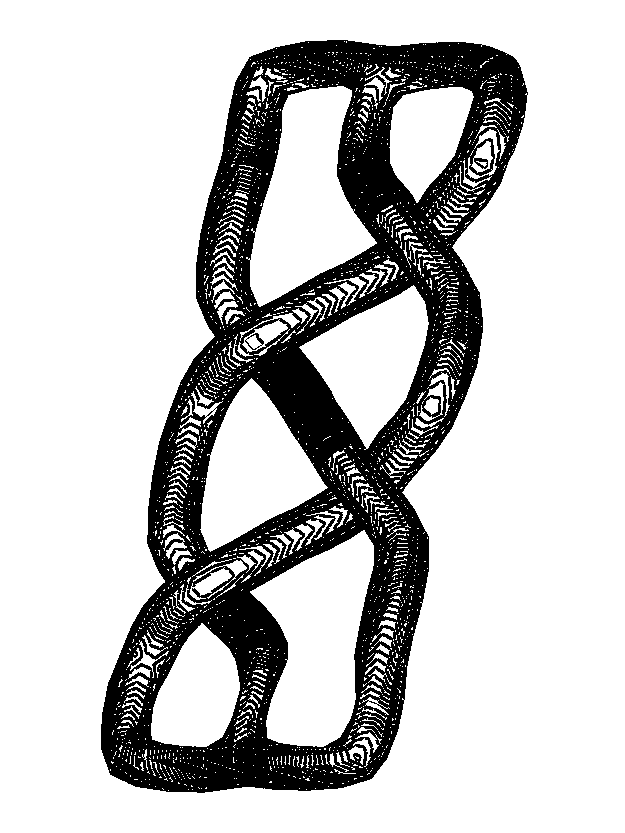
\includegraphics[width=0.5\textwidth]{braid_iso}
\end{figure}

\section{Installing the program}\label{section:installation}

The program can be built on your local machine by following these instructions:

\begin{enumerate}
\item{Download the program files as a zip archive from github, from 
\url{http://github.com/dannycalegari/wireframe}.}
\item{Unzip the archive on your local computer; this should create a new folder containing
the source files, some examples, the source for this manual (as a LaTeX file), and a
makefile.}
\item{The makefile assumes the user has the GNU c compiler ({\tt g++}) installed, and that the standard
X-windows include files and libraries are installed in the directories {\tt /usr/X11R6/include}
and {\tt /usr/X11R6/lib}. Edit these values if necessary.}
\item{Make the program from the command line with the command {\tt make}.}
\end{enumerate}


\section{Data formats}\label{section:data_format}

The program is run from the command line with the command {\tt ./wireframe -w filename}
or {\tt ./wireframe -g filename}. The two options are explained below.

\subsection{Reading a file in wire format}

A data file called {\tt filename} in {\em wire format} may be read in with the command 
{\tt ./wireframe -w filename}. This data file defines a triangular mesh (possibly with
boundary, possibly disconnected) by specifying adjacency data and location of vertices. 
Here is an example of a file in wire format:

\begin{center}
{\tt
\begin{tabular}{lll}
8 & & \\
3 & 3 2 1 &	1.0 -1.0 -1.0 \\
5 & 2 4 6 3 0 & -1.0 -1.0 -1.0 \\
5 & 3 5 4 1 0 & 1.0 -1.0 1.0 \\
5 & 1 6 5 2 0 & 1.0 1.0 -1.0 \\
5 & 2 5 7 6 1 & -1.0 -1.0 1.0 \\
5 & 3 6 7 4 2 & 1.0 1.0 1.0 \\
5 & 4 7 5 3 1 & -1.0 1.0 -1.0 \\
3 & 6 4 5 & -1.0 1.0 1.0 \\
1.0 0.0 0.0 & & \\
1.0 1.0 0.0 & &
\end{tabular}
}
\end{center}

The format is defined abstractly as follows:
\begin{enumerate}
\item{The first line of the file is a positive integer $v$ which specifies the number of vertices.}
\item{Vertices are labeled from $0$ to $(v-1)$.}
\item{The subsequent $v$ lines are the data associated to vertices, in order from $0$ to $(v-1)$. So
the second line of the file is the data associated to vertex $0$, and the $(v+1)$st line is the data
associated to vertex $(v-1)$.}
\item{The data associated to vertex $i$ is a triple $v_i$, $L_i$, $(x_i, y_i, z_i)$.}
\item{$v_i$ is a positive integer, which is the valence of vertex $i$, or the valence plus 1 if 
vertex $i$ is a boundary vertex.}
\item{$L_i$ is a list of $v_i$ distinct integers. At most one entry in $L_i$ can be $-1$; all other
entries must be non-negative, must be between $0$ and $v-1$, and must not be equal to $i$.
Only the cyclic order of the list is important. The cyclic
order of the entries corresponds to the neighbors of vertex $i$ in anticlockwise order. A $-1$
entry indicates the outward normal to the boundary, so if $\cdots j, -1, k \cdots$ appears
in $L_i$ in this cyclic order, where $j$ and $k$ are non-negative, then vertices $j,i,k$ are
consecutive on the boundary of the mesh (with positive orientation).}
\item{$(x_i,y_i,z_i)$ are real numbers, and denote the location in space of vertex $i$. In
practice these should have absolute value at most $1.5$.}
\item{The last two lines are the RGB color values for the outer and inner boundaries respectively.}
\end{enumerate}

This data should satisfy certain consistency checks. For instance, if vertex $i$ lists vertex $j$
as a neighbor, then vertex $j$ should list vertex $i$ as a neighbor. Also, the mesh should
consist of triangles. If the file fails these consistency checks, the program will exit with
an error.

\subsection{Reading a file in graph format}

A data file called {\tt filename} in {\em graph format} may be read in with the command 
{\tt ./wireframe -g filename}. This data file defines a graph by specifying adjacency data 
and location of vertices. The syntax of graph format is identical to wire format
{\em except} that a file in graph format has two additional lines coming before the RGB
color values for inner and outer boundaries,
each consisting of a single real number $e$, $i$ (in order).

A data file in graph format specifies a graph with straight edges. As with wire format,
the first line of the file specifies the number of vertices, and subsequent lines specify,
for each vertex in turn, its neighbors (taken in cyclic order) and its location. 
So as in wire format, the data associated to vertex $i$ is a triple $v_i$, $L_i$, $(x_i,y_i,z_i)$.
These data must satisfy the following conditions:
\begin{enumerate}
\item{$v_i$ must be at least $2$.}
\item{$L_i$ is a list of $v_i$ distinct integers. If one entry of $L_i$ is equal to $-1$, then
$v_i=2$ and the other entry must be non-negative. Otherwise every entry of $L_i$ must be
non-negative.}
\end{enumerate}

The program reads in the graph, and computes from it a triangular mesh (possibly with
boundary), obtained as the boundary of a tubular neighborhood of the graph. The
number $i$ is the thickness of the neighborhood near internal vertices, and $e$ is
the thickness of ``boundary'' vertices. A $-1$
entry in a list $L_i$ (necessarily of length 2) denotes a ``boundary'' vertex, which
will correspond to a boundary loop in the associated triangular mesh.

\section{Program interface}\label{section:interface}

Running the program on a file in consistent wire or graph format will open an X-window
and display the mesh, initially in wire frame outline. The $x$--$y$ coordinates of the
mesh and the screen agree; the $z$ coordinate points out of the screen towards the viewer.

The following keypress options are available.

\begin{itemize}
\item{[f] toggles between solid and wireframe. Solid can be in either shaded or isobar mode.}
\item{[v] toggles between verbose and silent. Verbose is mainly useful for debugging.}
\item{[i] toggles between {\tt shaded} and {\tt isobar} mode. {\tt Shaded} mode paints each triangle in 
exterior or interior color (depending on its orientation) with an intensity proportional to the
vertical component of the normal. {\tt Isobar} mode is black and white, and draws the level
sets of the $z$ coordinate which are integer multiples of some specified value.}
\item{[1/2] makes isobars sparser/denser. The default spacing is $0.01$. Each keypress multiplies
or divides the spacing by $1.1$.}
\item{[s] subdivides and smooths mesh. The subdivision adds one new vertex for each edge. The new vertex
is displaced in the normal direction to make the new surface ``rounder''.}
\item{[c] flows the surface by curvature. This is a very crude implementation of (combinatorial) mean
curvature flow which tries to equalize edge lengths.}
\item{[t] trim pyramids. A ``pyramid'' is a 3-valent vertex. Such vertices tend to give rise to
strange artefacts when smoothed or flowed; this command trims them off.}
\item{[arrow keys] to rotate mesh. Each keypress rotates by $0.1$ radians in the $x$--$z$ plane or
the $y$--$z$ plane.}
\item{[$+/-$] to make mesh bigger/smaller. Each kepress multiplies or divides the scale by $1.05$.}
\item{[e] for .eps output. The user will be prompted for a file name to write .eps output to.}
\item{[q] to quit.}
\end{itemize}

\section{Acknowledgements}
Danny Calegari is partially supported by NSF grant DMS 1005246. The program {\tt wireframe} is
released under the terms of the GNU GPL License version 3.0.

\medskip

\noindent Version 1.0 of {\tt wireframe} was released February 19, 2013 and is copyright Danny Calegari.


\end{document}